\documentclass{beamer}
\usepackage[spanish]{babel}
\usepackage[utf8]{inputenc}
\usetheme{AnnArbor}
\usecolortheme{crane}
\useoutertheme{shadow}
\useinnertheme{rectangles}
\usepackage{multicol}
\title[CMTC]{Cadenas de Markov en tiempo continuo}
\author[Santiago,Jesus,Fernando]{Santiago de Diego, Jesús Bueno, Fernando de la Cruz, Javier Ruiz}
\date{}
\begin{document}
\frame{\titlepage}

\AtBeginSection{
\begin{frame}
  \frametitle{Índice}
  \begin{multicols}{2}
  \tableofcontents[currentsection]
  \end{multicols}   
\end{frame}
}

\AtBeginSubsection{
\begin{frame}
  \frametitle{Índice}
  \begin{multicols}{2}
  \tableofcontents[currentsection,currentsubsection]
  \end{multicols}
\end{frame}
}

\section{Introducción}
\begin{frame}
    \frametitle{Introducción}
     Las cadenas de Markov son procesos de corta memoria en el sentido de que solo recuerdan el último estado visitado para decidir cual será el próximo.
     \newline
     \newline
     Este tipo de procesos estocásticos tienen mucho interés a la hora de modelar determinados fenómenos, como por ejemplo el tiempo de espera a un servidor en función de la tasa de llegada de los clientes.
  \end{frame}
  \begin{frame}
       \begin{block}{Definición de Cadena de Markov}
  		 El proceso $\{\mathbb{X}_n \}_{n\in \mathbb{N}}$ con espacio de estados $E$ es una cadena de Markov si:
$$P(\mathbb{X}_{n+1}=y \, | \, \mathbb{X}_n = x_n , \ldots , \mathbb{X}_0 = x_0)=P(\mathbb{X}_{n+1}=y \, | \, {\mathbb{X}_n=x_n})$$
  		\end{block}
  	\end{frame}
\begin{frame}
\frametitle{Diferencia con tiempo discreto}
La principal diferencia entre cadenas de Markov en tiempo discreto y tiempo continuo es, como dice el propio nombre, el tiempo.
\newline
\newline
En las cadenas de Markov en tiempo continuo, consideramos un $t\in T \subset \mathbb{R}$ mientras que en las cadenas de Markov en tiempo discreto, trabajamos con instantes de tiempo de la forma $t\in \mathbb{N}$.
\end{frame}

\section{Definición y propiedades}
\begin{frame}
    \frametitle{Definición y propiedades}
    Primero de todo presentamos dos definiciones equivalentes de Cadenas de Markov en tiempo continuo:
    \newline
    \begin{block}{Definición 1: Cadena de Markov}
Decimos que $\{\mathbb{X}_t\}_{t\geq 0}$, proceso estocástico en tiempo continuo es una Cadena de Markov en tiempo continuo si $\forall t,s\geq 0$ y $\forall i,j,x_u\in E$ con $0\geq u \geq s$, se cumple que:
$$P(\mathbb{X}_{t+s}=j \, | \, \mathbb{X}_s =i \, , \,  \mathbb{X}_u =  u \,\, \forall 0\leq u\leq s)=P(\mathbb{X}_{t+s}=j \, | \, \mathbb{X}_s = i)$$
    \end{block}

\end{frame}
\begin{frame}
    \begin{block}{Definición 2: Cadena de Markov}
    El proceso estocástico $\{\mathbb{X}_t \, , \, t\in [0,\infty]\}$ es una Cadena de Markov en tiempo continuo si para cualquier entero $n\geq 0$, cualesquiera $0\leq t_0 < t_1 < \ldots < t_{n+1}$ y $i_0,\ldots , i_n,i_{n+1}\in S$ se verifica:
$$P(\mathbb{X}_{t_{n+1}}=i_{n+1}\, | \, \mathbb{X}_{t_0}=i_0 , \ldots \mathbb{X}_{t_n}=i_n)=P(\mathbb{X}_{t_{n+1}}=i_{n+1}\, | \, \mathbb{X}_{t_n}=i_n)$$
    \end{block}
\end{frame}

\begin{frame}
Una vez vistas las dos definiciones anteriores estamos preparados para enunciar dos propiedades muy importantes de Cadenas de Markov de tiempo continuo:
\begin{block}{Primera propiedad}
$P(\mathbb{X}_{t_{n+h}}=i_{n+h}, h=1,\ldots m \, | \, \mathbb{X}_{t_k}=i_k, k=0,\ldots ,n)=P(\mathbb{X}_{t_{n+h}}=i_{n+h}, h=1,\ldots m\, |\, \mathbb{X}_{t_n}=i_n )$
\newline\newline
$\forall 0 \leq t_1< t_2, \ldots , < t_n+m\, , \forall i_k\in S, k=0,\ldots , n+m$
\end{block}
\begin{block}{Segunda propiedad}
$P(\mathbb{X}_{t_{n+h}}=i_{n+h}\, | \, \mathbb{X}_{t_k}=i_k \, ,  k=0,\ldots , n)=P(\mathbb{X}_{t_{n+h}}=i_{n+h}\, | \, \mathbb{X}_{t_n}=i_n)$
\end{block}
\end{frame}
\section{Probabilidades de transición}
\begin{frame}
    \frametitle{Probabilidades de transición}
    \begin{block}{Definición de Probabilidades de transición}
    Dada una CMTC $\{\mathbb{X}_t \, , \, t\in [0,\infty]\}$, definimos las probabilidades de transición como:
$$p_{ij}(s,t):=P(\mathbb{X}_t=j\, | \, \mathbb{X}_s=i), \ 0\leq s < t, \ \ i,j\in S$$
    \end{block}
    A partir de aquí supondremos que la CMTC es homogénea.
    \newline	\newline
     La probabilidad de ir del estado $i$ al estado $j$ no depende del instante de tiempo en el que se encuentra la cadena, es decir, $p_{ij}(s,t)$ no depende de $s$ y $t$, sólo depende de la diferencia $t-s$. Esto nos da pie a enunciar la siguiente propiedad:
  \end{frame}
  \begin{frame}
  \begin{block}{Propiedad}
  Podemos expresar las probabilidades de transición como:
 $p_{ij}(t)=P(\mathbb{X}_t=j\, | \, \mathbb{X}_0=i)=P(\mathbb{X}_{t+s}=j\, | \, \mathbb{X}_s=i)$
  \end{block}
  Además en la siguiente diapositiva presentamos otras tres propiedades muy importantes:
   \end{frame} 
   \begin{frame}
    \begin{block}{Propiedades}
\begin{enumerate}
\item Para cada $t\geq 0, \ \ p_{ij}(t)\geq 0, \ \ \forall i,j\in S$,
\item Para cada $t\geq 0, \ \ \sum\limits_{j\in S}p_{ij}(t)=1, \ \ \forall i\in S$,
\item Ecuación de \textit{Chapman-Kolmogorov}: 
$p_{ij}(s+t)=\sum\limits_{k\in S}p_{ik}(s)p_{kj}(t), \ \ \forall i,j\in S, \ \ \forall s,t\in[0,\infty)$.
\end{enumerate}
  \end{block} 
  \end{frame}
\subsection{Q-matriz}
\begin{frame}{Q-matriz}
\begin{block}{Definición de Q-matriz}
Dada una CMTC $\{\mathbb{X}_t \, , \, t\in [0,\infty]\}$, con matriz de transición $P(t)$. Se define la $Q$-matriz o generador infinitesimal como:
$$Q:=\lim_{t \to 0}\dfrac{P(t)-I}{t},$$
\end{block}
donde:
\begin{itemize}
\item $I$ es la matriz identidad del tamaño correspondiente
\item  $q_i$ es la \textit{razón de escape} del estado $i$
\item $q_{ij}$ es llamado \textit{razón de transición} del estado $i$ al $j$.
\end{itemize}
\end{frame}
\section{Ecuación de Kolmogorov}
\begin{frame}
    \frametitle{Ecuación de Kolmogorov}
    Esto es una introducción
\end{frame}

\section{Clasificación de los estados}
\begin{frame}
    \frametitle{Clasificación de los estados}
    Esto es una introducción
\end{frame}

\section{Teoremas límite}
\begin{frame}
    \frametitle{Teoremas límite}
    \begin{block}{Teorema Ergódico}
    Para una cadena de Markov irreducible se verifica:
	\begin{enumerate}
    \item Si todos los estados son recurrentes positivos:
$$\lim_{t\rightarrow\infty}p_{i,j}(t)=u_j>0 \, , \, \forall i,j\in S$$
Además $u=(u_j \, , \, j\in S)$ es la única distribución estacionaria de la cadena y $\displaystyle\lim_{t\rightarrow\infty}a_j (t)=u_j \, , \, \forall j\in S$. La distribución de probabilidad u es la solución del sistema $uQ=0$, siendo $Q$ la $Q$-matriz de la cadena.
\item Si todos los estados son recurrentes nulos o transitorios,
$$\lim_{t\rightarrow\infty}p_{ij}(t)=0\, , \, \forall i,j \in S\, ;\,\,\, \lim_{t\rightarrow\infty}a_j (t)=0\, , \, \forall j\in S$$
\end{enumerate}
    \end{block}
\end{frame}

\section{Relación con la teoría de autómatas}
\begin{frame}{Relación con la teoría de autómatas}
\begin{block}{Definición de Grafo de una CMTC}
$G=(E,U,W)$ es el grafo asociado a una CMTC sii:
\begin{itemize}
\item $E$ es el conjunto de estados de la cadena
\item $U$ es el conjunto de transiciones posibles (aristas)
\item $W$ es el conjunto de ponderaciones. Podemos verlo como el conjunto de valores de cada arista
\end{itemize}
Además $G$ es un grafo orientado, es decir, que tenemos en cuenta cual es el nodo origen y cual es el nodo destino.
\end{block}
\end{frame}
\begin{frame}
Aquí podemos ver un ejemplo de grafo de una CMTC:
\newline
\begin{figure}[h]
  \centering
    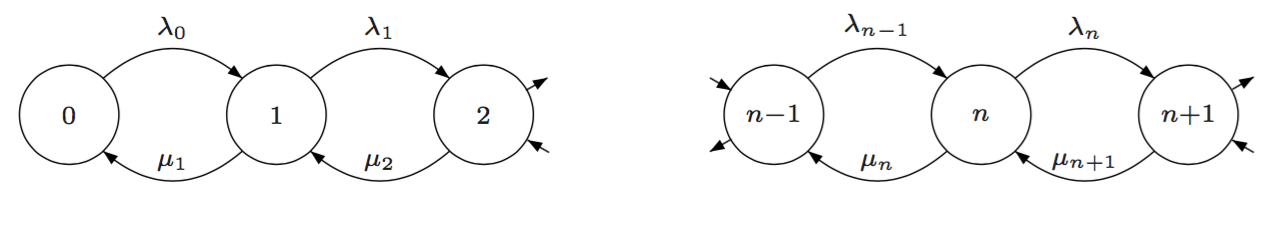
\includegraphics[width=0.9\textwidth]{img/grafo.png}
  \label{fig:ejemplo}
\end{figure}
Una vez vista la definición de grafo de una CMTC vamos a introducir la definición de autómata finito determinista:
\end{frame}
\begin{frame}
\begin{block}{Definición de autómata finito determinista}
Un AFD es una 5-tupla $(Q,\sum ,q_0,\delta,F)$ donde:
\begin{itemize}
\item $Q$ es un conjunto de estados
\item $\sum$ es un alfabeto
\item $q_0$ es el estado inicial
\item $\delta :Q\times\sum\rightarrow Q$ es la función de transición
\item $F\subseteq Q$ es el conjunto de estados finales
\end{itemize}
Además verifica que $\delta (q,a)=q_1$ y $\delta (q,a)=q_2 \Rightarrow q_1 \neq q_2$ y que no existen transiciones de la forma $\delta(q,\epsilon)$ donde $\epsilon$ es la cadena vacía
\end{block}
\end{frame}
\begin{frame}
Aquí podemos ver un ejemplo de AFD:
\newline
\begin{figure}[h]
  \centering
    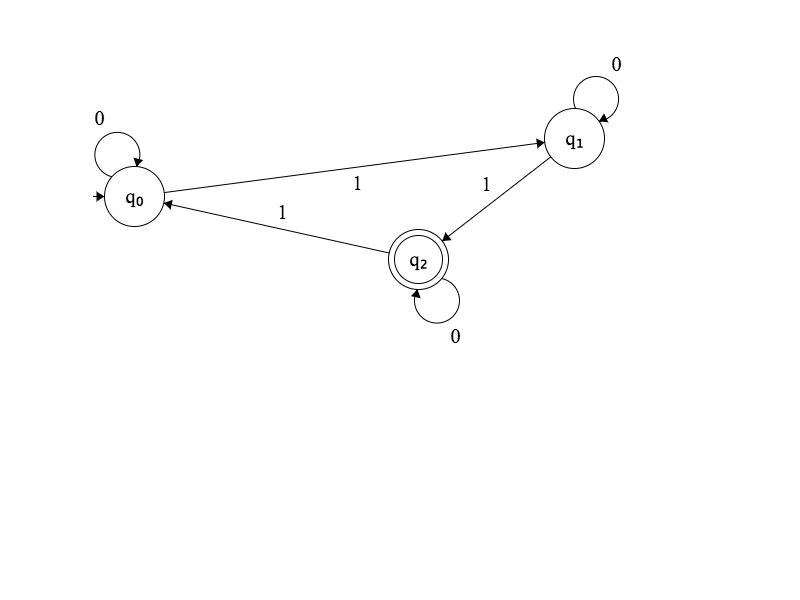
\includegraphics[width=0.9\textwidth]{img/afd.png}
  \label{fig:ejemplo}
\end{figure}
\end{frame}
\begin{frame}
En el ejemplo anterior podemos diferenciar:
\begin{itemize}
\item $Q=\{q_0,q_1,q_2 \}$
\item $\sum = \{0,1\}$
\item $q_0=q_0$
\item $\delta \, t.q$:
\\
$\delta(q_0,0)=q_0 \,\,\,\,\,\,\, \delta(q_1,0)=q_1\,\,\,\,\,\,\, \delta(q_2,0)=q_2$
\\
$\delta(q_0,1)=q_1 \,\,\,\,\,\,\,  \delta(q_1,1)=q_2 \,\,\,\,\,\,\,\delta(q_2,1)=q_0$
\item $F={q_2}$
\end{itemize}
\end{frame}
\begin{frame}
De manera intuitiva, podemos ver la relación entre el grafo de una CMTC y un AFD, sin más que considerar que este último tiene $F={\emptyset}$, es decir, no tiene estados finales.
\newline\newline
Además podemos ver la correspondencia: $Q=E\, ,\, \sum=W$ y $| \delta |=U$
\end{frame}
\section{Ejemplos}
\subsection{Ejemplo 1}
\begin{frame}
    \frametitle{Ejemplos}
    Esto es una introducción
\end{frame}
\begin{frame}
    \frametitle{Ejemplo 1}
    Esto es una introducción
\end{frame}
\end{document}
